\documentclass[12pt,a4paper]{report}

\usepackage[utf8]{inputenc} % pentru suport diacritice
\usepackage[english]{babel} % setări pentru limba română 
\renewcommand\familydefault{\sfdefault} % sans serif

\usepackage[margin=2.54cm]{geometry}	% dimensiuni pagină și margini
\usepackage{graphicx} % support the \includegraphics command and options

% formatting sections and subsections
\usepackage{textcase}
\usepackage[titletoc, title]{appendix}
\usepackage{titlesec}
\titleformat{\chapter}{\large\bfseries\MakeUppercase}{\thechapter}{2ex}{}[\vspace*{-1.5cm}]
\titleformat*{\section}{\large\bfseries}
\titleformat*{\subsection}{\large\bfseries}
\titleformat*{\subsubsection}{\large\bfseries}

\usepackage{chngcntr}
\counterwithout{figure}{chapter} % no chapter number in figure labels
\counterwithout{table}{chapter} % no chapter number in table labels
\counterwithout{equation}{chapter} % no chapter number in equation labels

\usepackage{booktabs} % for much better looking tables
\usepackage{url} % Useful for inserting web links nicely
\usepackage[bookmarks,unicode,hidelinks]{hyperref}

\usepackage{array} % for better arrays (eg matrices) in maths
\usepackage{paralist} % very flexible & customisable lists (eg. enumerate/itemize, etc.)
\usepackage{verbatim} % adds environment for commenting out blocks of text & for better verbatim
\usepackage{subfig} % make it possible to include more than one captioned figure/table in a single float
\usepackage{enumitem}
\setlist{noitemsep}

%%% HEADERS & FOOTERS
\usepackage{fancyhdr}
\pagestyle{empty}
\renewcommand{\headrulewidth}{0pt}
\renewcommand{\footrulewidth}{0pt}
\lhead{}\chead{}\rhead{}
\lfoot{}\cfoot{\thepage}\rfoot{}


\newcommand{\HeaderLineSpace}{-0.25cm}
\newcommand{\UniTextEN}{UNIVERSITY POLITEHNICA OF BUCHAREST \\[\HeaderLineSpace]
FACULTY OF AUTOMATIC CONTROL AND COMPUTERS \\[\HeaderLineSpace]
COMPUTER SCIENCE AND ENGINEERING DEPARTMENT\\}
\newcommand{\DiplomaEN}{DIPLOMA PROJECT}
\newcommand{\AdvisorEN}{Thesis advisor:}
\newcommand{\BucEN}{BUCHAREST}

\newcommand{\frontPage}[6]{
\begin{titlepage}
\begin{center}
{\Large #1}  % header (university, faculty, department)
\vspace{50pt}
\begin{tabular}{p{6cm}p{4cm}}

\includegraphics[scale=0.8]{pics/upb-logo.jpg} &
	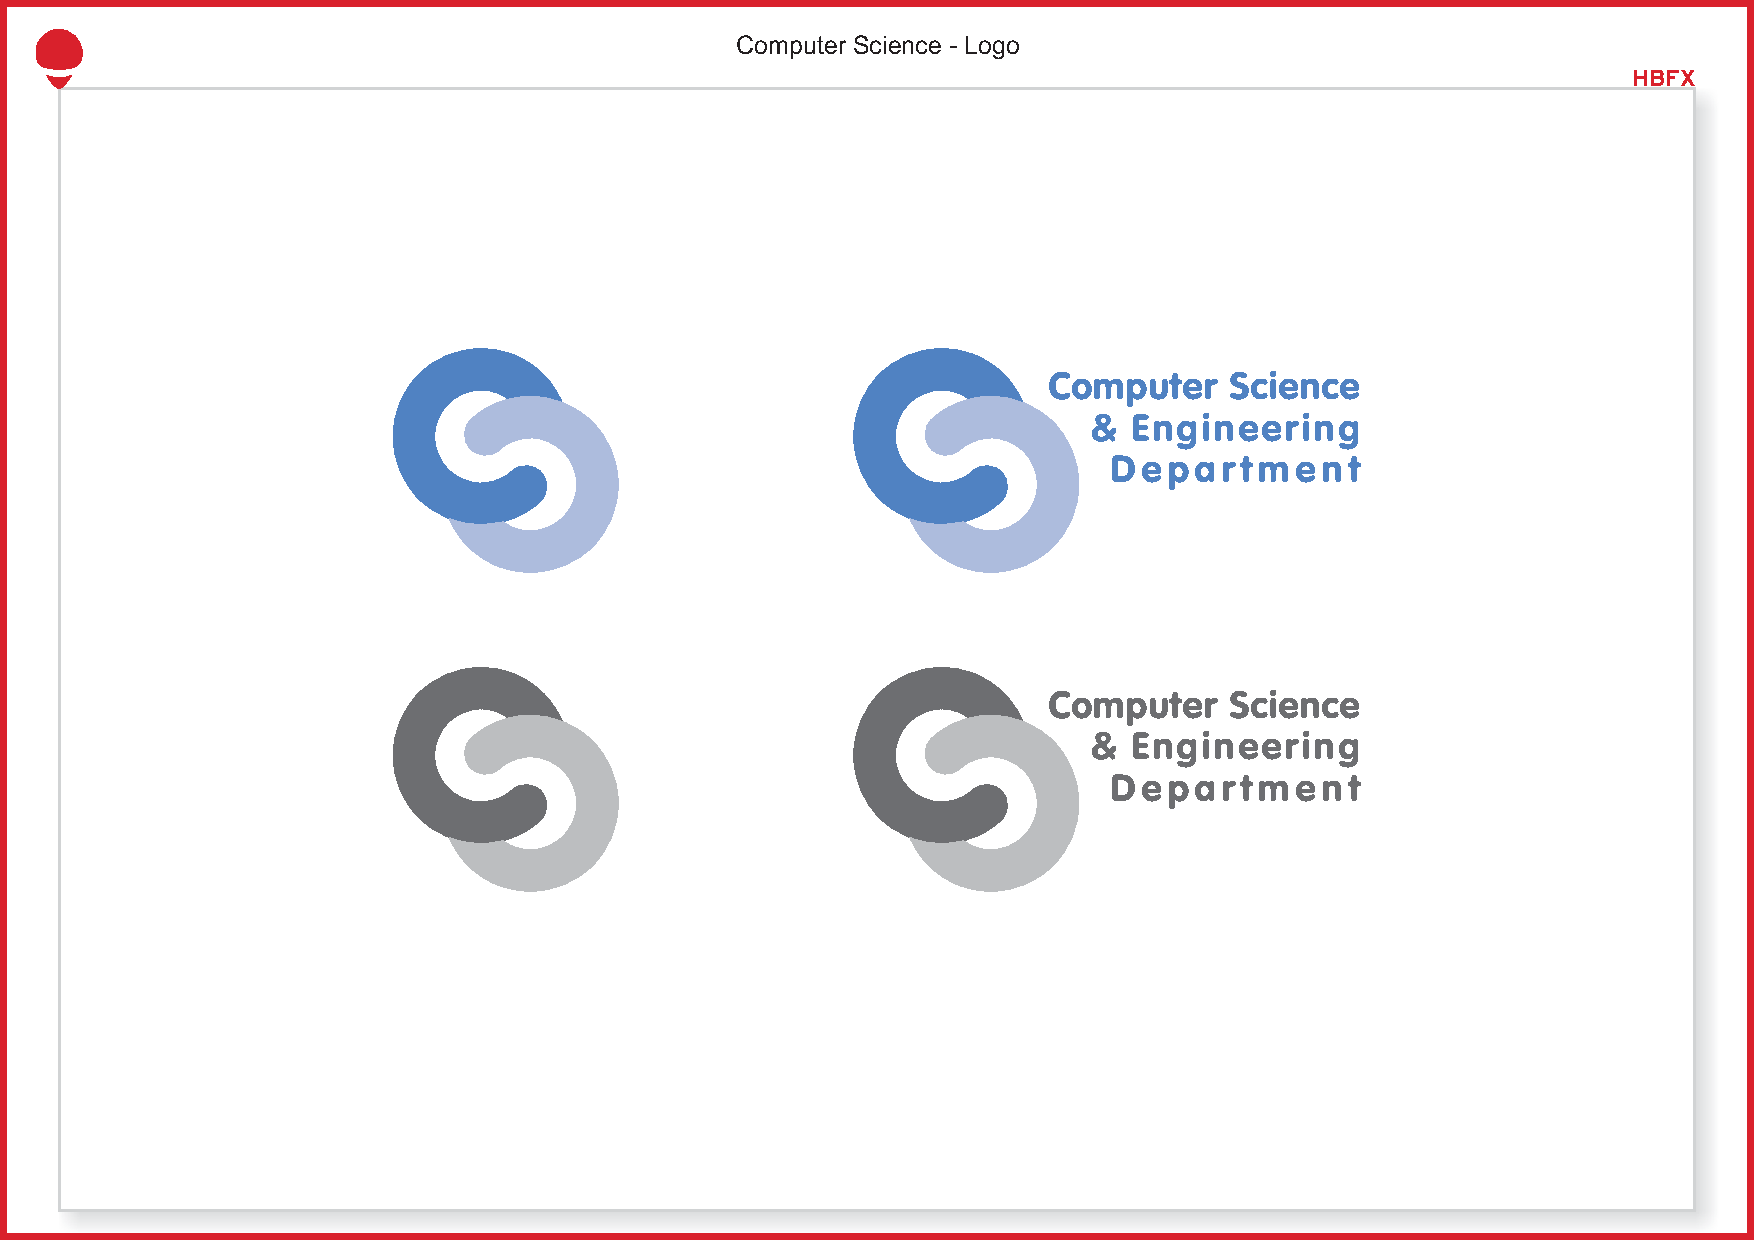
\includegraphics[scale=0.5,trim={14cm 11cm 2cm 5cm},clip=true]{pics/cs-logo.pdf}
\end{tabular}

\vspace{105pt}
{\Huge #2}\\                           % diploma project text
\vspace{40pt}
{\Large #3}\\ \vspace{0pt}  % project title
{\Large #4}\\                          % project subtitle
\vspace{40pt}
{\LARGE \Name}\\                   % student name
\end{center}
\vspace{60pt}
\begin{tabular*}{\textwidth}{@{\extracolsep{\fill}}p{6cm}r}
&{\large\textbf{#5}}\vspace{10pt}\\      % scientific advisor
&{\large \Advisor}                                    % advisor name
\end{tabular*}
\vspace{20pt}
\begin{center}
{\large\textbf{#6}}\\                                % bucharest
\vspace{0pt}
{\normalsize \Year}
\end{center}
\end{titlepage}
}

\newcommand{\frontPageEN}{\frontPage{\UniTextEN}{\DiplomaEN}{\ProjectTitleEN}{\ProjectSubtitleEN}{\AdvisorEN}{\BucEN}}

\linespread{1.15}
\setlength\parindent{0pt}
\setlength\parskip{.28cm}

%% Abstract macro
\newcommand{\AbstractPage}{
\begin{titlepage}
\textbf{\large ABSTRACT}\par
\AbstractEN \vfill
\end{titlepage}
}


%%%%%%%%%%%%%%%%%%%%%%%%%%%%%%%%%%%%%%%%%%%%%%%%%%   
%%
%%          End of template definitions
%%   
%%%%%%%%%%%%%%%%%%%%%%%%%%%%%%%%%%%%%%%%%%%%%%%%%%


%%% Puteți elimina aceste linii din lucrare, servesc numai pentru template.
\newcommand{\worktype}[1]{[\textit{#1}] }
\newcommand{\dezvoltare}{\worktype{Dezvoltare de produs}}
\newcommand{\cercetare}{\worktype{Cercetare}}
\newcommand{\ambele}{\worktype{Ambele}}
%%%


%%
%%   Campurile de mai jos trebuie modificate de autor. Modificati doar continutul, nu si numele fiecarei definitii
%%
\newcommand{\ProjectTitleEN}{Trading Bot}
\newcommand{\ProjectSubtitleEN}{Making an autonomous program that does the trading for you}
\newcommand{\Name}{Stanciu Stefan-Lucian}
\newcommand{\Advisor}{Prof. dr. ing. Radulescu Florin}
\newcommand{\Year}{2021}

% Setări document
\title{DIPLOMA PROJECT}
\author{\Name}
\date{\Year}

%%
%%   Campurile aferente rezumatului
%%

\newcommand{\AbstractEN}{With the evolution of technology and with the apparition of the internet, in this day and age, purchasing and selling financial products has never been easier. In the past investors would call their broker to make a trade for them. They could either visit or telephone their broker, but now everything is being done on an online trading platform. Using these platforms can have a lot of benefits, but there is also one big downside, which is if you want to make money constantly then you have to be online for quite some time each day, in order to not miss some good deals. My application, MoneyTrading, aims to offer the customers of a trading platform, xStation from XTB, a tool that will automatically make transactions for them based on the their preferences.}


\begin{document}

\frontPageEN

\begingroup
\linespread{1}
\tableofcontents
\endgroup

\AbstractPage


\chapter{Introduction}\pagestyle{fancy}
\section{Context}
Traditionally, if investors or traders wanted to make a trade, they would have had to call their brokerage firms with a purchase or sell request. The process of confirming such an important request was a long and tedious one, with multiple phone calls or meetings in which a lot of topics needed to be addressed. The subjects that were approached by both parties involved (broker and the investor) were about the market's price, the limit price, how long to keep the order open for, in what account to purchase the shares (if the client had multiple accounts) and if the investment representative would approve the commission costs for making the trade. A lot of time and effort was spent on making transactions in the past.

Today, with so many advancements in the digital era, increasingly more investors are choosing to use online trading platforms from the comforts of their home, at any time they want. Online trading, simply put, refers to buying and selling financial assets using proprietary trading platforms offered by a broker for DIY (do-it-yourself) investing. As high-speed computers and good internet connections were made more and more accessible to every citizen, in the mid to late '90s the use of online trading increased exponentially. On such platforms there were made available, to purchase or sell, all kinds of currencies, stocks, bonds, options, funds, EFTs (electronic funds transfers). As of today, some of the most popular assets in the online trading domain are currencies, cryptocurrencies, stocks, commodities and one of the largest financial market in the world, larger even then the stock market, is the foreign exchange or forex, with an average daily trading volume of 6.6 trillion US dollars, according to the 2019 Triennial Central Bank Survey of FX and OTC derivatives markets \cite{centralBank}.

Nowadays, anyone can start trading online, simply, by opening a demat (dematerialized account that provides the facility of holding shares and securities in an electronic format) and creating an online account on a trading platform, but, in order to have success in this domain, it also requires a lot of information about the markets and about the stocks as stated in \cite{marketWizards}. There's quite a wealth of mostly free information out there on the internet like financial articles, stock market books and website tutorials from which one can grasp the intricacies of this domain. Online trading can be a really great way to earn a daily income as well as plan for the future, if it is done right.

\section{The Problem} 
The advent of online trading platforms, came with a lot of benefits, but also with some negatives, to both investors and traders. For example, one benefit is the improvement in speed and simplicity of which transactions can be made, due to the lack of need for paper-based documents to be copied, filed for each transaction. Another benefit is that an investor can now monitor the changes in market's prices and his investments all the time, but this benefit can also become one of the main disadvantages of online trading platforms, because it requires a lot of dedication and a lot of attention, in order to not lose money and make a profit. Online trading, can become a full time job for some investors, even if they already have another career, because of the need to be online on the platform for quite a while, day after day, monitoring each change in the market's price, making all the right transactions at the right moments, just to not lose out on potentially important or lucrative trades. In other words, online trading can consume a lot of time from a person's life, and that's the main problem that I'm trying to solve with this project.        
\section{Objectives}
The main goal of MoneyTrading, my application, is to address the main problem that was presented above. This tool will target the investors that are using xStation, the online trading platform from XTB, and it aims to make online trading a way of earning extra money without the need to constantly be online, avoiding the need to continuously stare at some price graphs, just waiting for the right opportunity to present itself, in order to make a good/profitable transaction and also, to change, for the better, the trading experience into a less time consuming, side or main, activity. To achieve the objectives stated above, my project will have to ease the transactions process by automatically overseeing any changes in prices from the markets and by performing purchase or sell orders based on the user's preferences and the current state of the market. 
\section{Proposed Solution} 
My application, MoneyTrading, features an user interface from which the consumer can login into their account on xStation, using their password and account number. After a successfully authentication, they can select on which markets to start making transactions and, most importantly, how and when to make the desired transactions. These user's choices are processed by an algorithm that determines, based on the conditions from the input, if a trade request needs to be made. Once the trading information is provided then it is sent to xStation platform using XTB's API.
\section{Obtained Results}
The result is an autonomous program that does the trading for it's users. The transactions that it makes are entirely based on the user's input. It works on multiple markets at the same time, each market having it's own different options determined by the user. 
\section{Thesis Structure}
\begin{itemize}
	\item \textbf{Motivation and Requirements Analysis}: provides an insight into the motivation that made me develop my application, what it's functionalities are and what it's supposed to achieve
	\item \textbf{Related Work}: offers details about other products that have a similar purpose with my program and it also highlights some differences between the presented applications
	\item \textbf{Proposed Solution}: this chapter explores a detailed view of what technologies were used in the making of my project
	\item \textbf{Implementation Details}: provides an explanation of how the technologies from the previous chapter were used and how the algorithm works
	\item \textbf{Experimental Results}: presents the obtained results after using the application
	\item \textbf{Conclusion and Future Work}: this chapter gives an overview about what can be improved and what was gained from this project
\end{itemize}


\chapter{Motivation and Requirements Analysis}
\section{Motivation}
This project is motivated by the simple fact that making money on a trading platform takes a lot of time. Firstly, to have success in this domain, one has to learn and grasp the intricacies of markets and trades. Secondly, any investor will have to start making transactions whilst following closely almost every change in the market's prices, and these things require patience, dedication and a lot of free time. Therefore, my idea was to make an investor's life a bit easier by completely eliminating or by making one of the previous steps as less tedious as possible. We all know that knowledge is needed in almost every professional field, so I deemed that the first step is a mandatory one. That's why, inspired by a famous quote "Time is money" as stated by Benjamin Franklin in \cite{timeIsMoney}, I decided to develop a program that tries to make trading online as a side activity by getting rid of the need to frequently check for any modification in stocks, markets or any opened transactions.

\section{Requirements}
On the side of hardware requirements, in order to use my application entitled MoneyTrading, the consumer, has to posses a good and steady internet connection and a working computer or laptop. Software-wise, the user needs to have on his personal computer the latest Java version installed. Also the consumer is required to own an usable account on the trading platform xStation.

\section{Use Case}
Step 1: The user opens the application and then the first thing he sees is the authentication window in which he has to login using his account number and his password from the official platform xStation. At this stage, the user can choose between two types of accounts that are supported by the trading website which are demo and real account. The demo is a one month trial in which the consumer can experiment with different markets and values on the platform and the real account is where the money is, hopefully, being made. If the authentication is successful then he can advance to the next step, otherwise he has to reenter his credentials until an effective login.

Step 2:
After the confirmation of a successful authentication, the main window of the program appears from which the user can control on what markets and with what details to make future transactions.

Step 3:
After filling out the desired fields the user can then start the algorithm by pressing the button "Start placing orders", from the main window, and after that the consumer can sit back and let the magic happen, because the algorithm will start to make all the possible transactions based on the user's input at all the correct times. Furthermore, the user can add additional, optional, details like stop loss, trailing profit, the number of maximum orders, the time between transactions and a take profit value (all of these fields will be explained in the Proposed Solution chapter) to all future transactions by pressing the button "Activate additional fields" from the main window. The general flow of the application is displayed in Figure~\ref{fig:appflow}.
\begin{figure}[!ht]
	\centering
	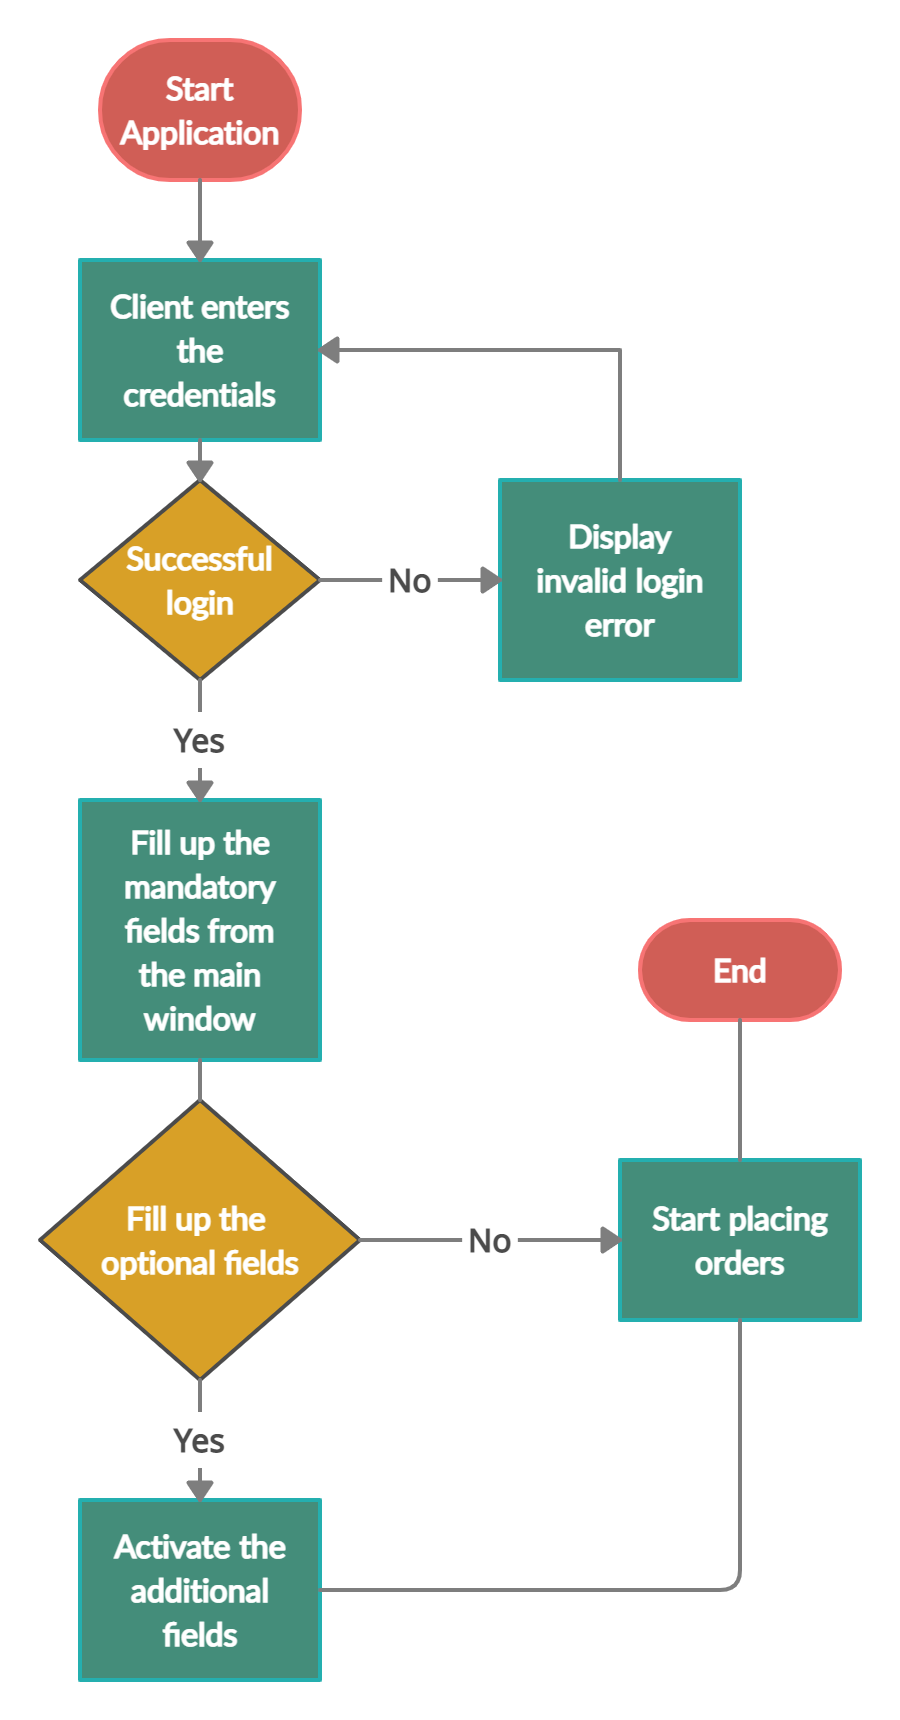
\includegraphics[width=7cm,height=10cm]{pics/appflow.png}
	\caption{The general flow of the application}
	\label{fig:appflow}
\end{figure}


\chapter{Related Work}
First of all, a trading bot is a software program that uses an API to interact with the consumer's exchange account and automatically execute trades based on its interpretation of the market data. This usually means that the bot will make a trade when market conditions meet a set of predefined and programmed criteria. Nowadays, with the explosion in popularity of digital currency, the most popular and the most sought after bots are the ones that automate cryptocurrency trading and they are called crypto bots. Even if the forex (foreign exchange) is the largest financial market in the world as stated in \cite{forex}, the availability and the demand for forex bots are way smaller compared to crypto bots, which is surprising considering that there are no guarantees when it comes to gains from forex and cryptocurrency trading. Moreover, there are 3 types of bots:
\begin{itemize}
	\item Arbitrage - a good way of explaining this type is by starting to define what arbitrage means and that is the simultaneous purchase and sale of the same financial asset in different markets, in order to make a profit from the slight differences in the asset's price. To simply put it, arbitrage takes advantage of the inevitable and imminent inefficiencies in markets and creates an opportunity for quite an almost risk-free profit for the investor. 
	As for this type of bot it represents a tool that examines prices across various exchanges and then executes trades in order to take advantage of markets' discrepancies.
	\item Historical - this type of tool examines and analyses past data prices in order to predict future changes in markets and to, possibly, come up with a trading strategy that would, theoretically, offer investors a boost in profits.
	\item Signal - this bot is programmed to execute trades based on signals triggered by a certain amount of numerical variation in trading volume or price.
\end{itemize}
As online trading became more and more popular so did these autonomous programs. There are many simple and reliable trading bots available to use that are obtainable by either free download, purchase or subscription. As for what these bots offer to traders is quite simple, they offer the capability to automate their trades, making their lives a whole lot easier while they wait for the program to make a profit. However, on many occasions, because of the unpredictable nature of markets, making a profit while using a bot isn't always the case. Most of these bots, while they automatically execute trades on a user's exchange account, they offer almost no control over their programmed strategy making them relatively useless for an advanced and experienced investor. These kind of bots can be compared to a mystery box, because the user doesn't always know what they are actually getting. The consumer has to rely on the creator's understanding of the market and programming skills that went into making the bot's strategy. As a result, the quality of these autonomous programs can vary from good, to poor, to an outright scam. Finding the right bot depends entirely on the user's needs and experience in the trading domain. Even so, any bot's strategy can be caught by unanticipated factors and events like an exchange hack, a flash crash or a rapid rise in price.
     

\section{Similiar Solutions}
\subsection{1000pip Climber System}
\textbf{1000pip Climber System}\footnote{\url{https://www.1000pipclimberea.com}} (see Figure~\ref{fig:pip}) is a completely mechanical system that operates on foreign exchange markets and it offers an advanced trading algorithm in a very to use package. It is purchasable for 97 US dollars. This is a signal based bot that monitors 6 currency pairs EUR/USD, EUR/JPY, AUD/USD, USD/CAD, USD/JPY, and USD/CHF. The algorithm that this bot uses was designed to identify key areas of supply and demand pressure zones. Once one of these areas is detected then a probability is determined, which indicates if the market's price will come out of the pressure zone. This probability is calculated by analyzing the price movement over short, medium and long periods of time. If the algorithm determines that the probability is high enough for the price to develop out of the pressure zone then a signal is sent to mark a potentially successful trade. These are all the details the developers shared about their algorithm and methodology. This is not a very customizable bot because its complexity is kept internal and there are almost no settings for the user to change. The interface is simple and clear so that anyone could understand it and easily use it.    
\subsection{Zenbot}
\textbf{Zenbot}\footnote{\url{https://github.com/DeviaVir/zenbot}} (see Figure~\ref{fig:zenbot}) is an open-source crypto trading bot. It doesn't have an interface and it is fully controlled by command line. It is built using modern technologies like Node.js and MongoDB. Zenbot can also be integrated with other services like Discord, IFTTT and Telegram in order to inform the user about any updates in trades. It's quite customizable, but as there is no interface it does require some technical skills. That being said, it does provide access to already made strategies or the user can build his own personal approach to trading. Zenbot requires a lot of attention from the consumers as they have to read its documentation and understand all the parameters before they can use it successfully. This tool was implemented as secure as possible, but it is always up to users to make sure that this free software is consistently updated and not badly configured or installed. Being an open-source, Zenbot, is maintained by its community which means that there is no guarantee for any assistance or feedback in case something goes wrong. 

\newpage
\begin{figure}[!htbp]
	\centering
	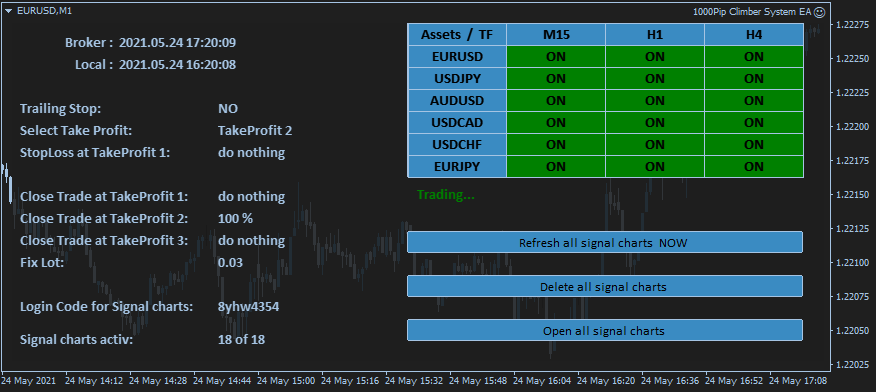
\includegraphics[width=16cm,height=9cm]{pics/1000PipClimberSystemEA.png}
	\caption{The 1000pip Climber System}
	\label{fig:pip}
	\bigskip
	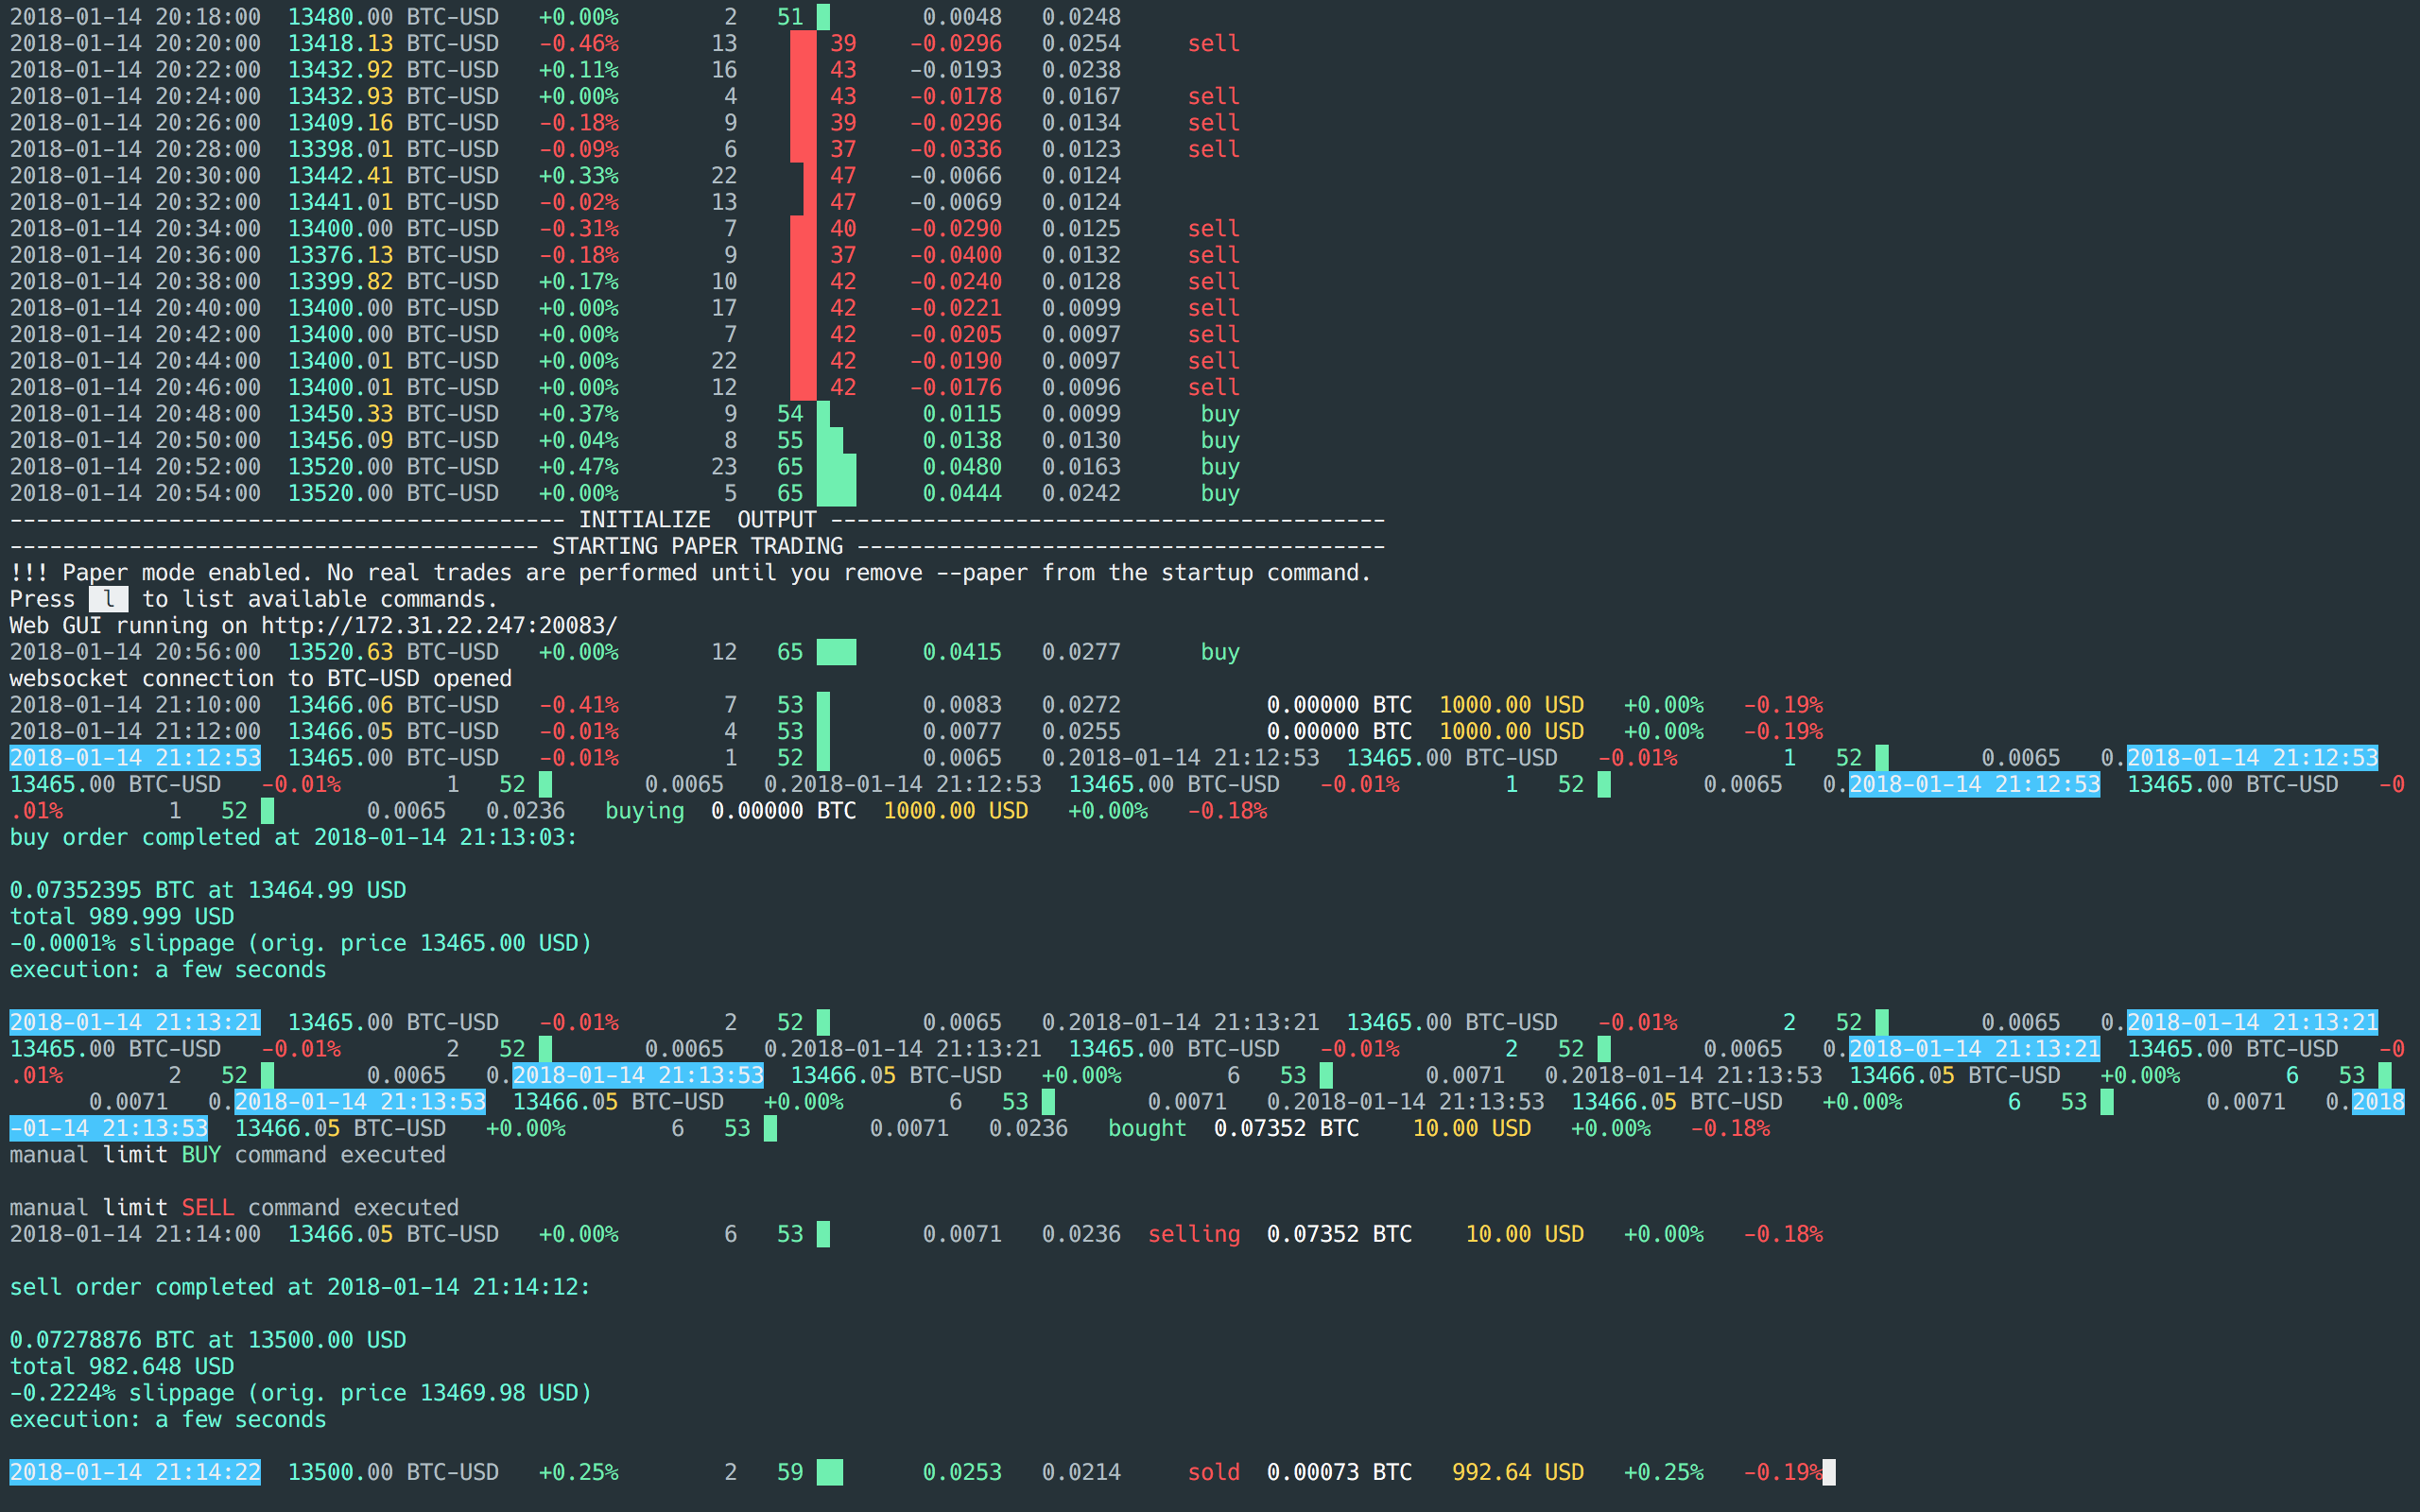
\includegraphics[width=16cm,height=9cm]{pics/zenbot.png}
	\caption{The Zenbot}
	\label{fig:zenbot}
\end{figure}

\newpage
\section{Comparison}
Because my application, MoneyTrading, is integrated with the XTB's API it can access any of its 2205 markets which include forex, indices, commodities, stock CFDs, ETF CFDs and crypto which is big advantage over the two bots that were presented above. My bot is a signal based program because it executes trades based on indicators triggered by a certain amount of fluctuation in price in a specific, customizable, period of time. MoneyTrading has an easy to understand interface with tool tips to help the user in figuring out what everything does, in contrast to Zenbot. The user can customize every value to future transactions just by filling out the fields dedicated to trade volume, take profit, stop loss, the maximum number of transactions to make on a selected market, trailing stop and the time between each future trade. MoneyTrading offers a level of customizability above the one offered by 1000pip Climber System.
\break
\renewcommand{\arraystretch}{1.5}
\begin{table}[th]\small\linespread{1}
	\begin{tabular}{l >{\raggedright\arraybackslash}p{3.5cm} >{\raggedright\arraybackslash}p{3.5cm} >{\raggedright\arraybackslash}p{3.5cm}}
		\textbf{Feature} & \textbf{1000pip Climber System} & \textbf{Zenbot} &\textbf{MoneyTrading} \\ [0.5cm]\hline
		\textbf{A pleasant interface} & Yes & No & Yes \\[0.5cm]\hline
		\textbf{Customizable} & No & Yes & Yes \\ [0.5cm]\hline
		\textbf{\textit{A plethora of markets}} & No & No & Yes \\ [0.5cm]\hline
		\textbf{Free} & No & Yes & Yes\\ [0.5cm]\hline
	\end{tabular}
	\caption{Comparing the features}
	\label{tab:comparsion}
\end{table} 

\chapter{Proposed Solution}
In order to make such an autonomous program I had to begin by building the interface. The user had to be able to login using his xStation account so I had to make a login window (see Figure~\ref{fig:login}) from which he could also choose the type of account, real or demo, he wanted to authenticate with. To also ease the user's access to his account I thought that a "Save credentials" checkbox would be a quality of life feature which would make the consumer's login go a little bit faster and effortless. After a successful login, the user would be presented with the main window (see Figure~\ref{fig:mainwindow}) which has the following mandatory input fields:
\begin{itemize}
	\item Market - this field is a drop down with all the available markets from the xStation trading platform. The user has to choose one valid market on which to start the algorithm that will automatically execute trades. 
	\item Price Difference - this is a TextField in which the user has to write a double type value. This number will become the value for which to look out for at each chosen market's price change.
	\item Time Interval - this is also a TextField and its value represents the interval of time in which to look out for the price difference at each market's price change.
	\item Trade volume - this field refers to the volume of currency that will be used for each future transaction. In other words, it represents how much the user wants to pay for each transaction.
\end{itemize}
The described fields above are mandatory for the algorithm because without any values it cannot execute any basic trades. There are also some optional fields for the user to further customize his approach to trading. These optional fields are all TextFields and they require a double type value:
\begin{itemize}
	
	\item Stop Loss (S/L) - this field represents a value that is either subtracted or added to the price of each transaction and its result can be defined as a price point where an advance order to sell the asset is triggered. This field is used to limit loss or gain in a trade. To better explain what this field does I feel that an example is needed:
	\begin{itemize}
		\item For a buy order - Stop Loss value is equal to the price of the index (market) at the time of placing the order from which the S/L value, written by the user in this field, is subtracted. \\
		For example: The inserted value for S/L is 30\$ and the buy order was executed at 950\$, then the stop loss value for this transaction will be set at 920\$.
		\item For a sell order - The difference here is that the S/L isn't subtracted from the index's price but it is now added. \\
		For example: The inserted value for S/L is 30\$ and the buy order was executed at 650\$, then the stop loss value for this transaction will be set at 680\$.
	\end{itemize}

	\item Take profit (T/P) - this field represents a value that is either subtracted or added to the price of each transaction and its result can be defined as a price point where the opened position will be closed. This field is used to maximize the profits. Just like in the Stop Loss's explanation an example would better demonstrate this field's use:
	\begin{itemize}
		\item For a buy order - Take Profit value is equal to the price of the index (market) at the time of placing the order from which the T/P value, written by the user in this field, is added. \\
		For example: The inserted value for T/P is 30\$ and the buy order was executed at 950\$, then the take profit value for this transaction will be set at 980\$.
		\item For a sell order - The difference here is that the T/P isn't added from the index's price but it is now subtracted. \\
		For example: The inserted value for T/P is 30\$ and the buy order was executed at 650\$, then the take profit value for this transaction will be set at 620\$.
	\end{itemize}

	\item Max Transactions - this field refers to the maximum number of transactions that will be made on the chosen market.
	
	\item Trailing Stop (T/S) - this field is percentage based and its purpose is to constantly check if the market's price moved towards the T/P that was set, multiplied by the percentage provided, for the opened orders, then the values stop loss and take profit are updated based on the current index's price. To better illustrate the definition I present the following example:
	\begin{itemize}
		\item For a buy order - The inserted value for T/S is 50\%, the T/P was set at 30\$ and the buy order was executed at 950\$ so the take profit value is 980\$. When the index's price reaches 965\$ then the values for take profit and stop loss for the current transaction are updated using the latest price. 
		\item For a sell order - The inserted value for T/S is 50\%, the T/P was set at 30\$ and the buy order was executed at 650\$ so the take profit value is 620\$. When the index's price reaches 635\$ then the values for take profit and stop loss for the current transaction are updated using the latest price.
	\end{itemize}
	The provided numbers for T/P and S/L by the user stay the same and in order to activate the trailing stop for future transactions the fields take profit and stop loss are mandatory.
	
	\item Time/Transactions - it represents the minimum time between each future transaction.
\end{itemize}
There is also an output window (see Figure~\ref{fig:output}) from which the user can track every update, made by the algorithm, like each new transaction, each new change in an order's stop loss and take profit and also when the number of opened trades reaches the maximum transactions value, if there is one.

\section{Technologies}
The interface was all built in Java and for its development I used the technologies presented below. 
\subsection{AWT API}
Java AWT (Abstract Window Toolkit) is an API made for developing graphic user interfaces or window-based applications in Java. AWT was made with the intent to call the native platform, which refers to operating systems, subroutine for creating components such as text areas, buttons, drop downs etc. For instance, an AWT graphic user interface with a button and a text area would have a completely different look and feel across distinct platforms like Linux, Windows and Mac operating system.This happens because these platforms have different looks and feels for their native buttons and text areas, meaning that AWT directly calls their native platform subroutine that creates these components. To simply put it, a software program that was made using AWT would look like a Windows type of application if it was executed on Windows, but the same application would look like a Linux program if it ran on an UNIX operating system.

Nowadays, because of its platform depended nature AWT is rarely used. Its components are all constructed by the operating system on which the application runs. The hierarchy of Java AWT classes are given below in Figure~\ref{fig:awt}.
\begin{figure}[!ht]
	\centering
	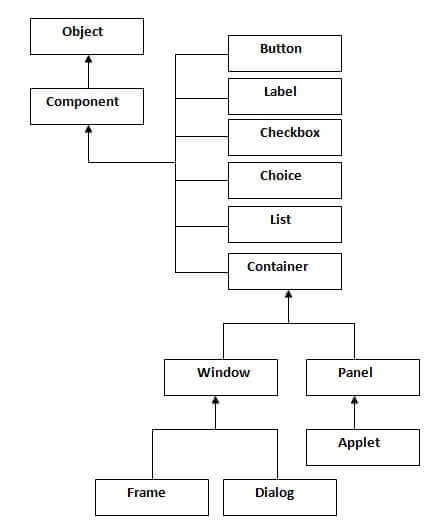
\includegraphics[width=10cm,height=10cm]{pics/awthierarchy.jpg}
	\caption{The hierarchy of Java AWT classes}
	\label{fig:awt}
\end{figure}
\newpage
Containers are components from AWT API that incorporate other components like buttons, labels, check boxes etc. There are four types of containers available:
\begin{itemize}
	\item Window: it doesn't have borders, menu bars and a title.
	\item Frame: as shown in the hierarchy above, the frame is a subclass of the window class, but it has everything that the window container is missing. It is the most used container when developing Java applications and it can have components like buttons, labels, text boxes etc.
	\item Panel: it doesn't have bars, a title or borders and it represents a generic container for holding other components.
	\item Dialog: it has a border, a title and it is a subclass of the window class, but it cannot exist without an associated instance of a frame.   
\end{itemize}
AWT has only two layouts available and are the following:
\begin{itemize}
	\item Flow: it is the default layout and when it is applied on a frame or panel it would force the contained components to be placed in a row form that are aligned in center by default.  
	\item Border: it is a more complex layout due to the fact that it has five regions and any new component must be added in one of these regions (PAGE\_START, LINE\_START, CENTER, LINE\_END, PAGE\_END). 
\end{itemize}
AWT is the foundation upon which Swing is made, meaning that Swing is an improvement in every way and it manages to be a platform independent GUI API.
\subsection{Swing API}
Swing API is a part of the Java Foundation Classes (JFC) that is used to ease a developer's life while creating front end/GUI applications using Java. As I said before, it is built on top of AWT API and it is platform independent. Swing API is based on a MVC architecture:
 \begin{itemize}
 	\item Model: it represents a component's data.  
 	\item View: it is the graphical illustration base on a component's data.
 	\item Controller: this element takes the input from the user's view and reflects the changes in the component's data
 \end{itemize}
Owing to the fact that Swing is based on the MVC architecture it comes with the following benefits:
\begin{itemize}
	\item Light Weight: Swing's components are independent of the platform that they are used on, therefore the API doesn't rely on operating system calls in order to build and render its visual components. The only thing that it uses is just Java. 
	\item Rich Controls: in addition to familiar components such as buttons, check boxes and labels, Swing provides several advanced components such as tabbed panel, trees, tables, lists etc.
	\item Highly Customizable: every component can be visually customized due to the fact that the appearance doesn't affect the functionality.
	\item Pluggable look-and-feel: this GUI's look and feel is changeable at run time just by using different available values.    
\end{itemize}
Every Swing graphic user interface recognizes three main aspects:
\begin{itemize}
	\item UI Elements - these represent the core of every interface and they are exactly what a consumer sees and interacts with in the application. 
	\item Layouts - these dictate how every component from a frame or panel are organized and placed in the application.
	\item Behavior - it defines what happens with every intractable component when used by the consumer.
\end{itemize}
The hierarchy of java swing API is given below in Figure~\ref{fig:swing}.
\begin{figure}[!ht]
	\centering
	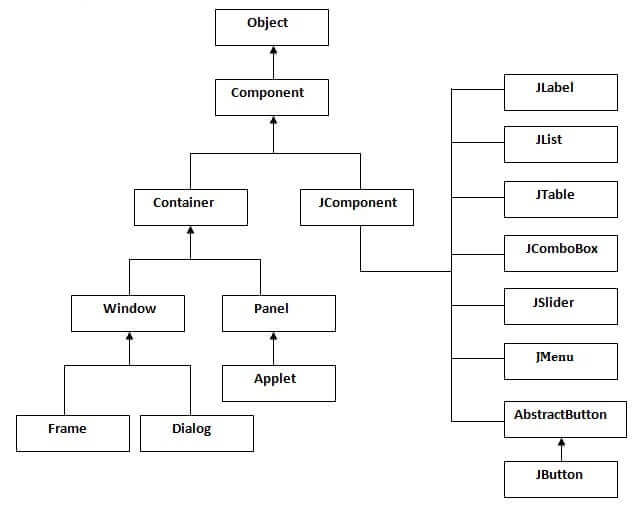
\includegraphics[width=12cm,height=10cm]{pics/swing.jpg}
	\caption{The hierarchy of Java Swing API}
	\label{fig:swing}
\end{figure}
\newpage
One of the most important things in a GUI is the user interface interaction. In Java, each user's interaction with a component is signaled by an event which describes that the state of the component has changed. As an example, clicking a button, typing a character in a text area or selecting an item from a drop down are all interactions that cause an event. There are two types of events:
\begin{itemize}
	\item Foreground - these are the types of events that are triggered by a human interaction with a graphical element like a button or a scroll bar. 
	\item Background - these events are generated by a hardware or system malfunction, by a flaw in the software code or by the completion of an operation.
\end{itemize}
In order to take advantage of this events and control what happens when they are triggered, there is, in Java, an event handling mechanism that specifies an action to take when an event occurs. Java uses the Delegation Event Model to handle the apparition of such events and this model has two key participants:
\begin{itemize}
	\item Source: it serves as the object that triggered the event and it needs to provide information to the handler about the action that just occurred.  
	\item Listener: it is also known as the event handler and it is responsible for developing a response to the event. 
\end{itemize}
The benefit of this model is that the logic which generates and handles events is totally separated by the user's interface logic. Another advantage is that the event handlers have to be registered with the component that will be responsible for generating the event, meaning that if the user finds himself in a situation where there are multiple buttons on the same frame and he pushes one, only the associated listener will receive the event notification and will trigger the appropriated response for that button.
In contrast to the layouts offered by the AWT API, Swing comes with five new layouts for even further customization:
\begin{itemize}
	\item Card: this layout makes it that each component in a container will be treated as a card and only one card can be visible at a time.  
	\item Grid: it arranges the frame's or panel's contained components in the form of a rectangular grid.
	\item Spring: it positions the components based on a set of constraints. 
	\item Grid Bag: this layout has the capability of aligning the components vertically and horizontally without depending on components having the same size.  
	\item Group: it groups elements hierarchically.
\end{itemize}
This technology was the most used in making my application's interface because it was way more customizable than the AWT API. 
\section{XTB's API}
In order for my program to communicate with the xStation platform I used the free XTB's API\footnote{\url{http://developers.xstore.pro/api/documentation.html}}. It provides the necessary means to request and get data from the main trading platform. The communication protocol that is utilized by this API uses a JSON format.\\
The general flow of the application using XTB's API is presented in Figure~\ref{fig:flow}.
\begin{figure}[!ht]
	\centering
	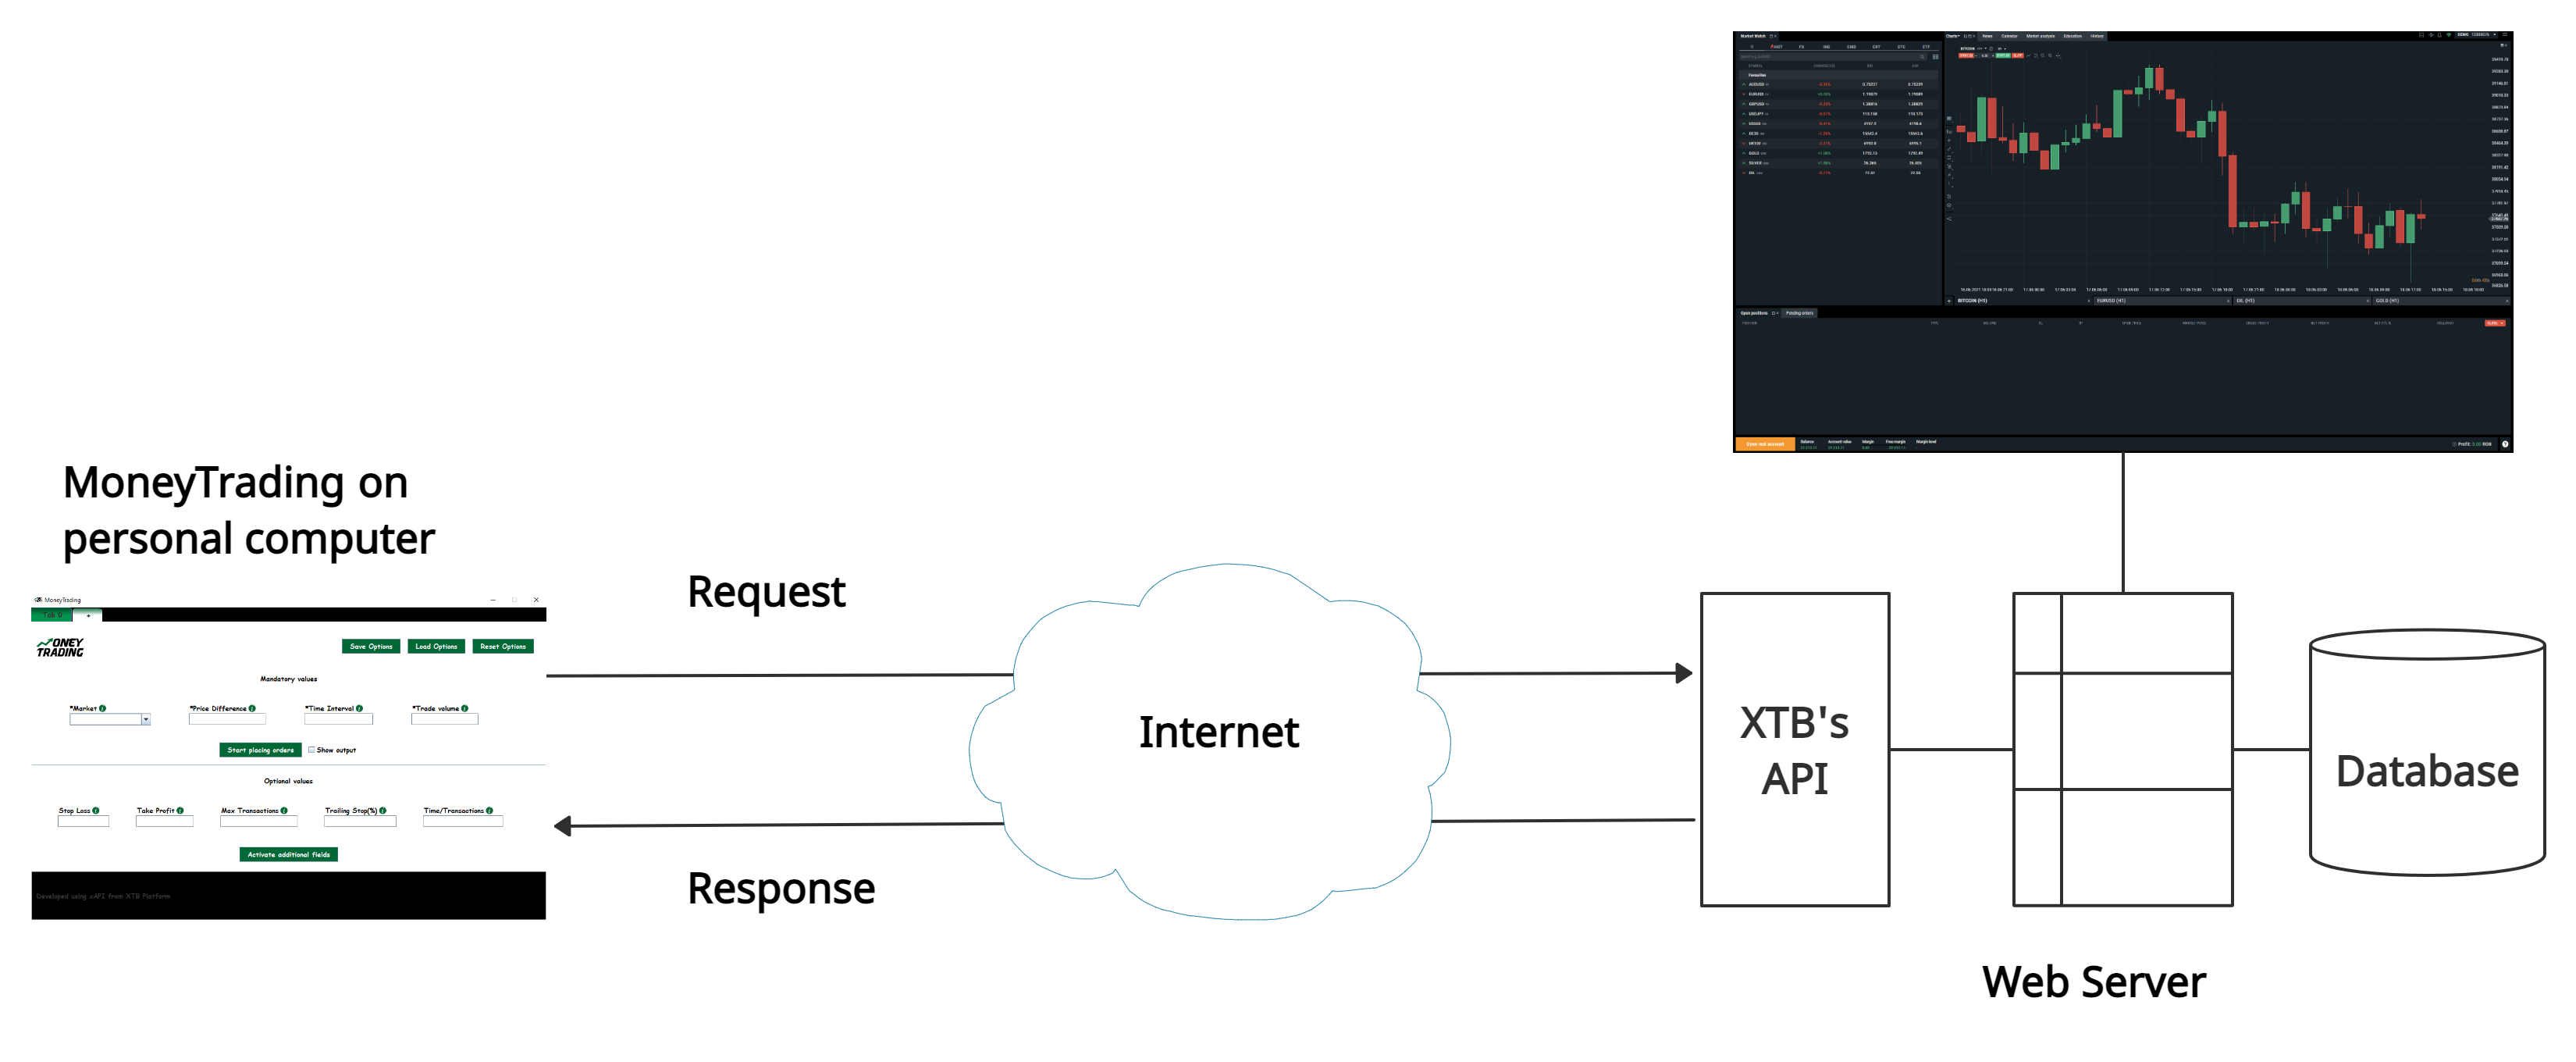
\includegraphics[width=16cm,height=8cm]{pics/flow.png}
	\caption{The general flow of the application}
	\label{fig:flow}
\end{figure}


\chapter{Implementation Details}

\section{Building the Interface}
\subsection{Login window}
To start making my autonomous trading program I had to make a clean and easy to understand interface. In achieving this I used Swing and AWT API. The login window contains two text fields, one for the account number and one for the password, a checkbox for saving the credentials and two buttons for selecting the type of the account which the user wants to authenticate on. In order to save the credentials I had to take the values from the two text fields and then save them into a file, so that at the next start up of the application the two text fields would have as default values the saved credentials. If the authentication isn't successful, then a message is displayed on the window for the purpose of warning the user. Once the credentials are valid, then the login window closes and the main window of the application opens up.

\subsection{Main panel}
Firstly, I had to consider how to arrange nine text fields and buttons in order to make it look good and not very cluttered. To pull this off, in a frame container, I made a main panel that used the Box Layout from Swing API and then created six other panels that would be contained by the main panel. The Box Layout made it that these panels would stack one on top of each other. These six panels are:
\begin{itemize}
 	\item Header: which contains the MoneyTrade's logo and three buttons for saving the current user's configuration "Save Options", loading a saved configuration "Load Options" and one for resetting all the text fields "Reset Options". For this panel I used the Border Layout from AWT API, because I wanted my logo to be on the far left side of the main panel (LINE\_START) and the buttons to be on the far right of the screen (LINE\_END).   
 	\item Simple order: it contains all the mandatory fields, all arranged on a row and in order to achieve such a placement I used the Flow Layout of which I changed it's default center alignment to a left alignment. Above each text field there are labels with tool tips which contain a short description of the fields. To pair the each label with its corresponding field I made small panels that used the Box Layout in which I introduced a label and a text field. After that I added these panels in the simple order panel, which automatically arranged the panels in a row.    
 	\item Place order: it's made out of a toggleable button "Start placing orders" that starts the algorithm and a checkbox that opens the output window or not. For this I used the Flow Layout, but now I left the default alignment on.  
 	\item Advanced order: it contains all the optional fields and the layout is the same as the one from the simple order panel.
 	\item Activate optionals: this is made out of just a toggleable button that introduces the optional values into the algorithm. It doesn't have any layouts, it's just a simple panel.
 	\item Footer: just a decorative panel with a label which states that the application was developed using the XTB's API. 
\end{itemize}
Each field, besides the market, needs to have an above zero double type value introduced, otherwise the user is warned that the value isn't a valid one. The "Start placing orders" cannot be toggled on until all the mandatory fields are filled out with valid values. The "Save Options" button opens up a new frame (see Figure~\ref{fig:saveload}) in which there are two buttons and a text field. To save the current configuration of the fields then the user has to enter a non-empty string for the file's name, otherwise the user is warned that the introduced name isn't a valid one. The two buttons from this window are "Close" which is self-explanatory and "Save" which creates a new file that contains all the values from the current configuration. The "Load Options" initiates a new window (see Figure~\ref{fig:saveload}) which contains two buttons "Close", "Load" and a drop down with all the saved configurations. Once the user decides on which configuration to use and selects it then he has to click the "Load" button in order to fill up the fields with the saved values. The two windows that open up after pressing the two buttons explained above, were built the same, meaning that both of them have a main panel that uses a Box Layout and that contains two other panels, one that consists of either a text field or a drop down and the other panel which utilizes the Flow Layout, that has two buttons. "Reset Options" has a pretty straightforward functionality and that is to clear out all the fields. If the check box "Show output" is checked then after pressing "Start placing orders" the output window opens up.

\subsection{The output window}
This frame was made with the purpose of tracking each change that happens due to the algorithm working. This window is made out of a main panel that has a Box Layout in which there are two other panels:
\begin{itemize}
	\item Notifications Area: which contains a text area in which every new notification will be displayed and a scroll pane that automatically scrolls down if the notifications are overflowing the text area.
	\item Options: this has three buttons in a Flow Layout with center alignment:
	\begin{itemize}
		\item Close: it is self-explanatory what this does.
		\item Pause Output: this is a toggleable button which is set as default on the value off and when it is on it makes that no new notification will be displayed in the text area, otherwise the normal flow of displaying notifications is resumed.
		\item Show Price Updates: another toggleable button which is set as default on the value off and its functionality is to make every price change be counted as a new notification.
	\end{itemize}
\end{itemize}

\subsection{The main frame}
This represents the container in which the main panel is. One big feature for my application that was surely needed was the possibility of having my algorithm work on multiple markets at the same time. For achieving this in the interface, I made the frame a tabbed pane, meaning that the frame could have multiple tabs opened, each for a different market with all new distinct values. What gave me the idea of having tabs was the fact that every modern browser has multiple tabs on which the user can have different websites opened at the same time. Each new tab consisted in a new main panel as shown below in Figure~\ref{fig:tabs}.
\begin{figure}[!ht]
	\centering
	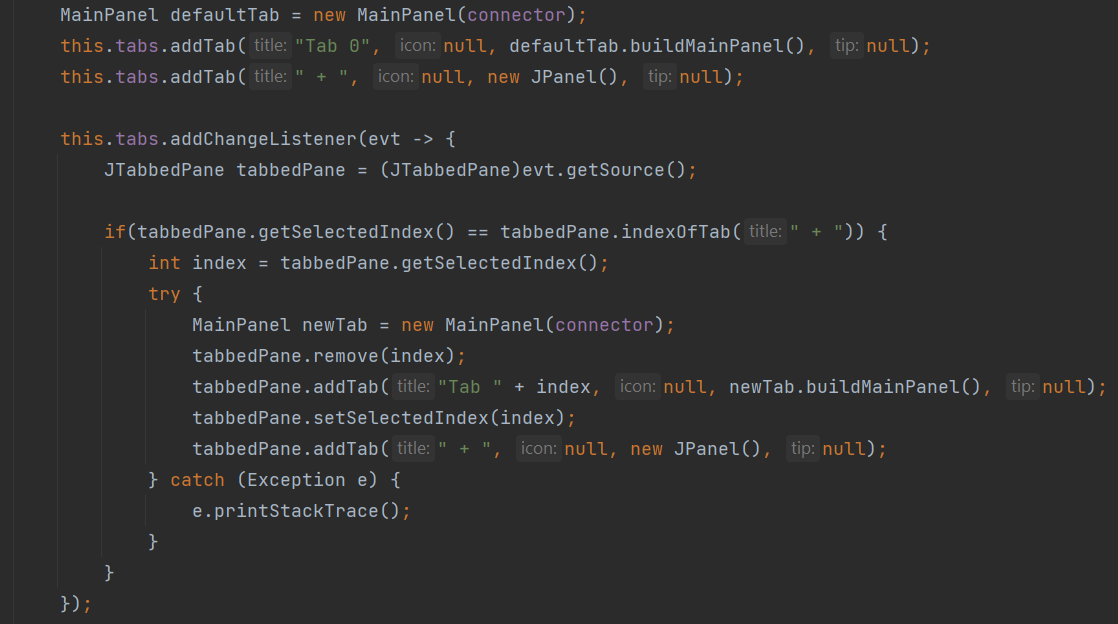
\includegraphics[width=13cm,height=8cm]{pics/tabs.png}
	\caption{Tabs code example}
	\label{fig:tabs}
\end{figure}

\subsection{The logo}
To add a more personal touch to the application I decided to make a logo in Adobe Illustrator, which is a graphical editor made by Adobe Systems. Because my program was called MoneyTrading, I tried to create a logo that would fit. The result can be seen in Figure~\ref{fig:logo}.
\begin{figure}[!ht]
	\centering
	
\includegraphics[width=10cm,height=6cm]{pics/logo.png}
	\caption{MoneyTrading Logo}
	\label{fig:logo}
\end{figure}

\subsection{Events}
To make my interface user interactible, each button, text field, check box and drop down that I used has an event listener attached to it. Every handler has a different purpose, based on its connected component, and they vary from having some simple functionalities, like changing a label or a boolean variable or just calling a method, to holding a more complex and important block of code, like having to collect the input's user and starting a thread based on those values while also checking that the variables are valid.  

An example on how an event listener is linked to a component is shown below in Figure~\ref{fig:events}.

\begin{figure}[!ht]
	\centering
	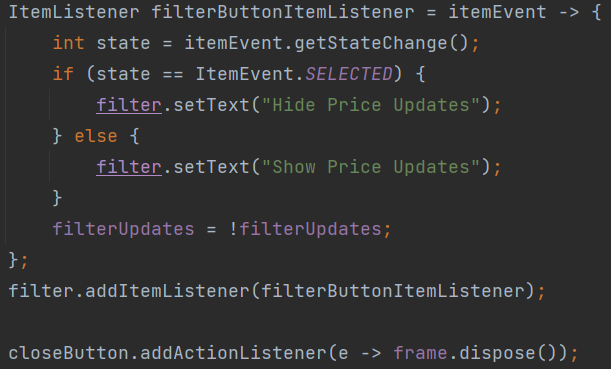
\includegraphics[width=10cm,height=6cm]{pics/events.png}
	\caption{Events code example}
	\label{fig:events}
\end{figure}

\section{The Algorithm}
The main idea of the algorithm is that every change in a market's price is saved for a specified amount of time (time interval field) in a Hash Map with the key of type double for saving the price and a value of type long for maintaining at which point in time this pair expires. An example can be seen in Figure~\ref{fig:prices}.
\begin{figure}[!ht]
	\centering
	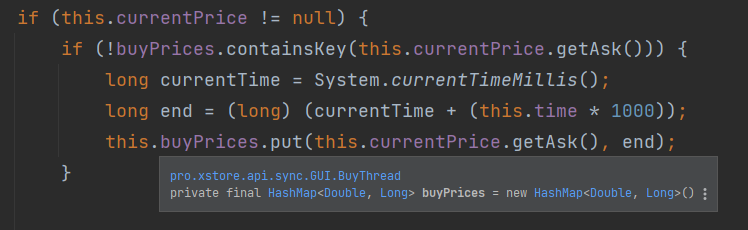
\includegraphics[width=13cm,height=4cm]{pics/prices.png}
	\caption{Hash Map Prices}
	\label{fig:prices}
\end{figure}
\\
If the Hash Map isn't empty then we iterate through it, comparing all the added keys with the current market's price checking if the price difference, submitted by the user, has been met or surpassed. If the price difference condition was met then a trade request will be sent to xStation using the API. Such a request can have all the optional fields that were completed by the user. The response received from the trading platform can have three status codes like ACCEPTED, REJECTED, and PENDING. An earlier point that I made was about the possibility of having my algorithm work on multiple markets at the same time and for accomplishing this task I decided to work with threads. In total I have five threads that are declared for each main panel:
\begin{itemize}
	\item Main Thread: which controls all of the other threads, meaning that it can pass on all of the submitted fields to all threads and it can start or stop them when an event is triggered. 
	\item Price Updates: this is just for constantly monitoring the market's price and checking if the maximum number of transactions was reached, if it was set.
	\item Buy Thread: this is dedicated to just making purchases, because of the fact that buy and sell prices are different, meaning that the formulas for take profit, stop loss and price difference are distinct from a sell order.
	\item Sell Thread: at this point the main purpose of this one is self-explanatory.
	\item Trailing Stop (Ts): this was made to constantly look out and make updates in the stop loss and take profit values of opened transactions. It also counts the number of trades that are opened on the selected market.   
\end{itemize}
Because of the API's limitation regarding the fact that a user can only send requests in 200ms intervals, otherwise the connection would be dropped, I needed to make sure that two different transactions requests couldn't be sent at the same time. For the purpose of resolving this problem I used a Reentrant Lock which would limit the access of making a transaction to just one thread at a time. This lock was used only in the threads that could send order requests and it was declared in the main thread on account of this being the one that controlled all of the other threads. Now, if a thread would fulfill the price difference condition, at first, it would have to check if the lock is acquired or not. After a successful trade request each thread needs to unlock the synchronization mechanism.
\newpage
An example of using the Reentrant Lock is displayed below in Figure~\ref{fig:lock}.
\begin{figure}[!ht]
	\centering
	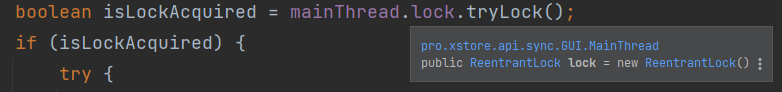
\includegraphics[scale=0.7]{pics/lock1.png}
	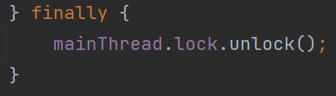
\includegraphics[scale=0.7]{pics/lock2.png}
	\caption{Using the Reentrant Lock}
	\label{fig:lock}
\end{figure}
\\
Of course, this wasn't enough to avoid the problem of having the connection dropped, because the lock would just make the trade requests become sequential and if a thread would finish processing a request and then another thread would send a request all in the 200ms time frame then the connection would be dropped. So, a small delay after each trade was surely needed to avoid this problem. In accomplishing this I used an Atomic Long value which is a variable that is written to memory, so that each change is visible to other threads. The scope of this value is to add a delay after each transaction which is verified by every thread before placing another order. Needless to say, this value needed to be updated, by a default delay of 250ms or by the user's time/transactions value, after each request before unlocking the synchronization mechanism.
Below, in Figure~\ref{fig:delay}, is an example of the atomic variable.
\begin{figure}[!ht]
	\centering
	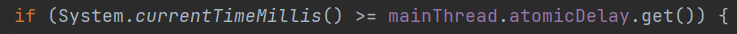
\includegraphics[scale=0.7]{pics/delay1.png}
	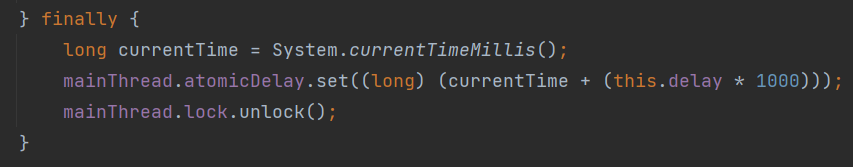
\includegraphics[scale=0.7]{pics/delay2.png}
	\caption{Using the Atomic Delay}
	\label{fig:delay}
\end{figure}
\\
In order to count the number of opened orders for the max transactions field I worked with an atomic integer which is updated after each new, successful trade request. If this value reaches the submitted user's limit then the buy and the sell threads are paused until the number of current transactions becomes lower than the set limit. Trailing Stop thread continues to run, because this only modifies the take profit and stop loss values for the already opened trades.

If the user runs out of funds while the algorithm is running then a new window will pop up to notify the consumer as seen in Figure~\ref{fig:nofunds}. When this frame opens up it generates a warning sound, making it more obvious. At the event of having no more funds then the buy and sell threads are stopped indefinitely until an algorithm restart is triggered by pressing again "Start placing orders".  

\subsection{Choosing the right design pattern}
Because the 

\chapter{Experimental Results}
\section{Interface Screenshots}
\begin{figure}[!ht]
	\centering
	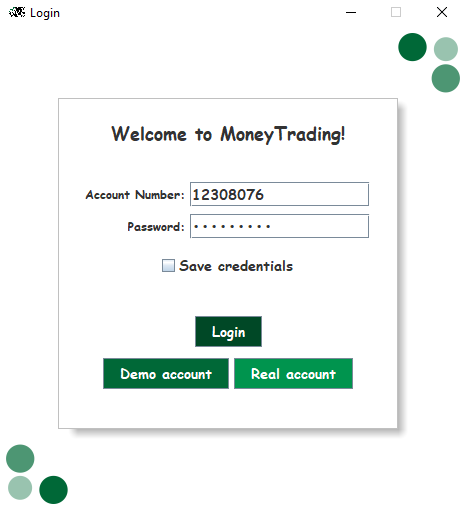
\includegraphics[width=5cm,height=5cm]{pics/login.png}
	\caption{The login window}
	\label{fig:login}
\end{figure}
\begin{figure}[!ht]
	\centering
	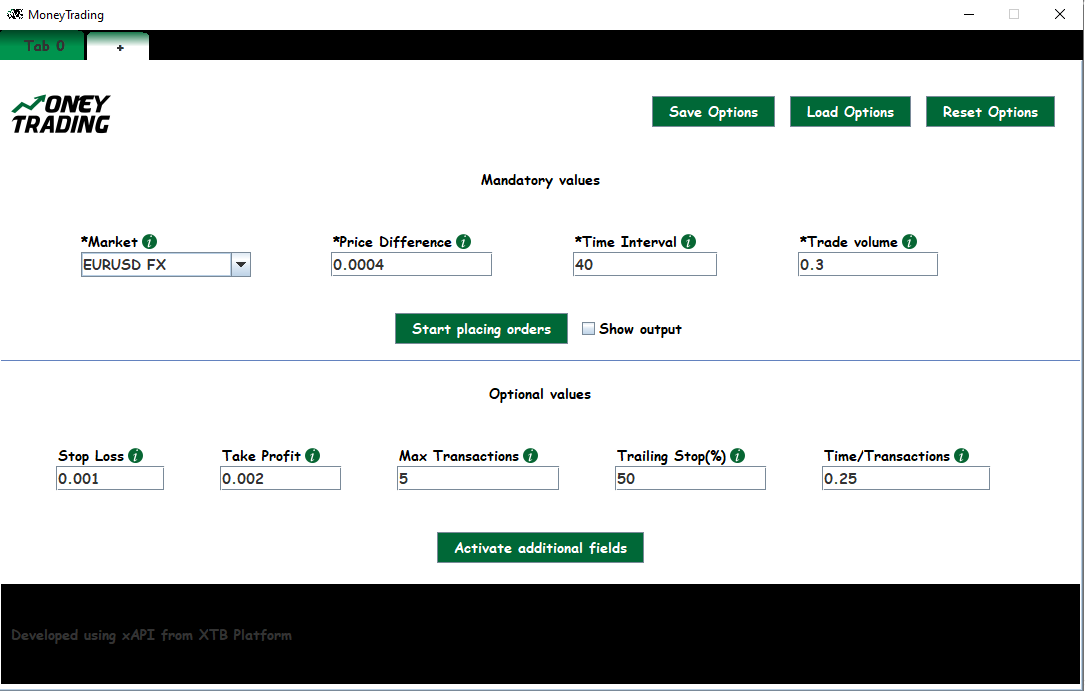
\includegraphics[width=16cm,height=10cm]{pics/mainwindow.png}
	\caption{The main window}
	\label{fig:mainwindow}
\end{figure}
\begin{figure}[!ht]
	\centering
	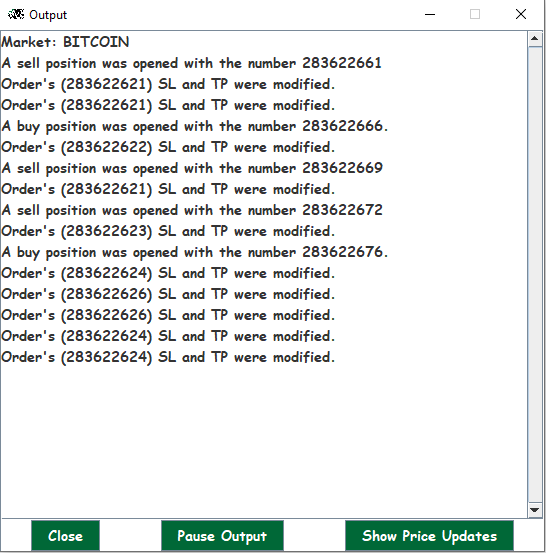
\includegraphics[width=10cm,height=10cm]{pics/output.png}
	\caption{The output window}
	\label{fig:output}
\end{figure}

\begin{figure}[!ht]
	\centering
	\subfloat[][\centering]{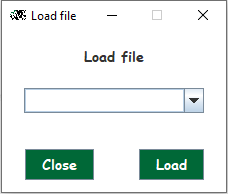
\includegraphics[width=5cm]{pics/load1.png} }
	\qquad
	\subfloat[][\centering]{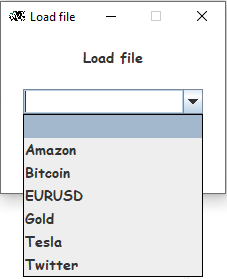
\includegraphics[width=5cm]{pics/load2.png} }
	\qquad
	\subfloat[][\centering]{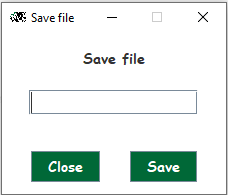
\includegraphics[width=4cm]{pics/save.png} }
	\caption{The load and save windows}
	\label{fig:saveload}
\end{figure}

\newpage
\section{Results}
Acest capitol trebuie să răspundă, în principiu, la 2 întrebări și să se încheie cu o discuție a rezultatelor obținute. Cele doua întrebări la care trebuie sa se răspundă sunt:
\begin{enumerate}
	\item  \textbf{Merge corect?} (Conform specificațiilor extrase în capitolul 2); 
Evaluarea dacă merge corect se face pe baza cerințelor identificate în capitolele anterioare. 

	\item Cât de \textit{Bine} merge / cum se compară cu soluțiile existente? (pe baza unor metrici clare). 
Evaluarea cât de \textit{Bine} merge trebuie să fie bazată pe procente, timpi, cantitate, numere, \textbf{comparativ cu soluțiile prezentate în capitolul 3}. Poate fi vorba de performanță, overhead, resurse consumate, scalabilitate etc. 
\end{enumerate}

În realizarea discuției, se vor utiliza tabele cu procente, rezultate numerice și grafice. În mod obișnuit, aici se fac comparații și teste comparative cu alte proiecte similare (dacă există) și se extrag puncte tari și puncte slabe. Se ține cont de avantajele menționate și se demonstrează viabilitatea abordării / aplicației, de dorit prin comparație cu alte abordări (dacă acest lucru este posibil). Cuvântul cheie la evaluare este ``metrică'': trebuie să aveți noțiuni măsurabile și cuantificabile. În cadrul procesului de evaluare, explicați datele, tabelele și graficele pe care le prezentați și insistați pe relevanța lor, în următorul stil: ``este de preferat ... deoarece …''; explicați cititorului nu doar datele ci și semnificația lor și cum sunt acestea interpretate. Din această interpretare trebuie să rezulte poziționarea proiectului vostru printre alternativele existente, precum și cum poate fi acesta îmbunătățit în continuare.

Criterii pentru calificativul \textit{Ne\textit{Satisfăcător}}: 
\begin{itemize}
	\item Aplicația este testată dar rulează pe calculatorul studentului, nu există posibilități de testare, nu a fost validată cu clienți / utilizatori;
	\item Nu au fost realizate comparații cu alte sisteme similare.
\end{itemize}

Criterii pentru calificativul \textit{Satisfăcător}: 
\begin{itemize}
	\item \dezvoltare  Există teste unitare și de integrare, există o strategie de punere în funcțiune (deployment), există validare minimală cu clienții / utilizatorii.
	\item \cercetare Principalele componente și soluția în ansamblu au fost evaluate din punct de vedere al performanței, însă nu sunt folosite seturi de date standard, există unele erori de interpretare a datelor.
	\item \ambele Discuție minimală asupra relevanței rezultatelor prezentate, comparație minimală cu alte sisteme similare.
\end{itemize}

Criterii pentru calificativul \textit{Bine}: 
\begin{itemize}
	\item \dezvoltare Teste unitare și de integrare, instrumente de punere in funcțiune (deployment) utilizate și care arată lucru constant de-a lungul semestrului, lucrare validată cu clienții / utilizatorii, produs în producție.
	\item \cercetare Componentele și soluția în ansamblu au fost evaluate din punct de vedere al performanței, folosind seturi de date standard și cu o interpretare corectă a rezultatelor.
	\item \ambele Discuție cu prezentarea calitativă și cantitativă a rezultatelor, precum și a relevanței acestor rezultate printr-o comparație complexă cu alte sisteme similare.
\end{itemize}

\chapter{Conclusion and Future Work}
În acest capitol este sumarizat întreg proiectul, de la obiective, la implementare, si la relevanta rezultatelor obținute. În finalul capitolului poate exista o subsecțiune de ``Dezvoltări ulterioare''.

Criterii pentru calificativul \textit{Ne\textit{Satisfăcător}}: 
\begin{itemize}
	\item	Concluziile nu sunt corelate cu conținutul lucrării;
\end{itemize}

Criterii pentru calificativul \textit{Satisfăcător}: 
\begin{itemize}
	\item	Concluziile sunt corelate cu conținutul lucrării, însă nu se oferă o imagine asupra calității și relevantei rezultatelor obținute;
\end{itemize}

Criterii pentru calificativul \textit{Bine}: 
\begin{itemize}
	\item	Concluziile sunt corelate cu conținutul lucrării, și se oferă o imagine precisa asupra relevantei și calității rezultatelor obținute în cadrul proiectului. 
\end{itemize}

% Asa se specifica folosirea unui fisier cu referinte bibliografice:
\bibliographystyle{plain}
\bibliography{bibliography}



\end{document}